\documentclass[12pt]{article}

% =========================
% PACKAGES
% =========================
\usepackage[a4paper,margin=1in]{geometry}
\usepackage{amsmath,amssymb,physics}
\usepackage{graphicx}
\usepackage{hyperref}
\usepackage{setspace}
\usepackage{enumitem}
\usepackage{tikz}
\usepackage{bm}
\usepackage{mathtools}

\setstretch{1.2}

% =========================
% TITLE
% =========================
\title{\textbf{Cyclical, Nested Cosmology with Persistent Gravitational Topology}\\
\large Dark matter as gravitational memory; black holes as temporal archives; cosmic structure as inherited constraint geometry}
\author{}
\date{}

\begin{document}
\maketitle

% =========================
\section*{Abstract}

We propose a speculative framework in which the universe is a \emph{nested, cyclical} system whose large-scale structure is governed by \textbf{persistent gravitational topology} rather than continuously novel initial conditions.

Topology is encoded at an early epoch, preserved and amplified by a collisionless metric component interpreted here as dark-matter geometry, and revealed by baryonic matter as a late-arriving tracer. Black holes are reinterpreted as \textbf{temporal mirror inversions}: surface-bound archives encoding the past worldlines of absorbed matter as horizon data.

% =========================
\section{Introduction}

Standard cosmology explains structure growth but leaves unresolved the origin of large-scale topology, the nature of dark matter, and the fate of information. This thesis reallocates explanatory roles rather than introducing new entities.

\begin{quote}
The universe does not invent structure every morning; it unfolds it.
\end{quote}

% =========================
\section{Early Encoding of Topology}

Inflationary perturbations encode a constraint graph of peaks, filaments, saddles, and voids. This is not a blueprint for galaxies, but a topological skeleton limiting later evolution.

We model the progression as:

\begin{center}
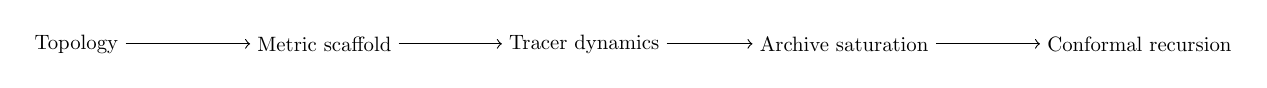
\begin{tikzpicture}[scale=0.75, transform shape]
\node (A) at (0,0)  {Topology};
\node (B) at (4.2,0) {Metric scaffold};
\node (C) at (8.6,0) {Tracer dynamics};
\node (D) at (13,0)  {Archive saturation};
\node (E) at (18,0)  {Conformal recursion};

\draw[->] (A) -- (B);
\draw[->] (B) -- (C);
\draw[->] (C) -- (D);
\draw[->] (D) -- (E);
\end{tikzpicture}
\end{center}

% =========================
\section{Dark Matter as Persistent Metric Geometry}

Dark matter is treated here not as exotic particles nor cross-universe gravity, but as long-lived curvature modes: \textbf{gravitational memory} inherited across cosmic epochs.

\begin{itemize}
\item Explains smooth halos and filaments
\item Explains robustness of the cosmic web
\item Requires no new interactions
\end{itemize}

We decompose the metric as

\[
g_{\mu\nu} = \bar{g}_{\mu\nu} + h_{\mu\nu}^{(b)} + h_{\mu\nu}^{(p)}
\]

where $h^{(p)}$ represents persistent curvature modes (the dark matter candidate) that satisfy

\[
\frac{d}{dt} h^{(p)} \approx 0
\]

% =========================
\section{Baryons as Tracers}

Baryonic matter is dissipative and late-arriving. It statistically settles into pre-existing attractors, revealing rather than creating structure.

Geodesic motion holds:

\[
\frac{D u^\mu}{D\tau} = 0
\]

with entropy production $\dot{S} > 0$.

% =========================
\section{Nested Branching and Degeneracy}

Fine-scale histories may branch into near-identical realizations. These branches do not interact; they become indistinguishable as entropy compresses degrees of freedom.

Microhistories form equivalence classes under coarse-graining:

\[
\Gamma_i \sim \Gamma_j \quad \text{if} \quad D(\Gamma_i,\Gamma_j) < \epsilon
\]

% =========================
\section{Black Holes as Temporal Mirror Archives}

A black hole is not a container in space but a \textbf{mirror in time}. The event horizon functions as an index surface encoding absorbed worldlines. The interior represents compressed, inverted ordering—not a forward narrative.

Horizon entropy remains

\[
S = \frac{A}{4G\hbar}
\]

interpreted as archive capacity. Worldlines map to horizon state:

\[
\mathcal{W} \rightarrow \mathcal{H}
\]

\begin{quote}
A black hole is a surface-written archive of everything that fell into it.
\end{quote}

% =========================
\section{Horizon Merging and Convergence}

As black holes merge and expansion isolates regions, micro-historical differences collapse into equivalence classes. Convergence occurs through loss of distinguishability, not interaction.

Archive merging:

\[
\mathcal{H}_{12} = \mathcal{H}_1 \oplus \mathcal{H}_2
\]

Differences compress via entropy increase.

% =========================
\section{Conformal Inversion and Cosmic Recursion}

The far-future horizon-dominated state becomes conformally equivalent to an inverted initial condition, allowing topological inheritance across cycles.

As $T \to 0$, scale becomes irrelevant. We apply the conformal mapping

\[
g_{\mu\nu} \to \Omega^2 g_{\mu\nu}
\]

so the late state can serve as an effective new initial condition.

% =========================
\section{Implications}

\begin{itemize}
\item Dark matter as gravitational memory
\item Cosmic web as standing topology
\item Black holes as archival endpoints
\item Cycles as re-expression, not replay
\end{itemize}

% =========================
\section{Falsifiability}

The framework fails if early-epoch topology does not statistically correlate with late-time lensing structure, or if large-scale coherence contradicts inheritance of curvature modes.

Prediction: correlation between early curvature and late lensing

\[
\rho = \text{corr}(\Phi_{\text{early}}, \kappa_{\text{lensing}})
\]

Framework falsified if $\rho \approx 0$.

% =========================
\section{Visual Model of Recursion}

\begin{center}
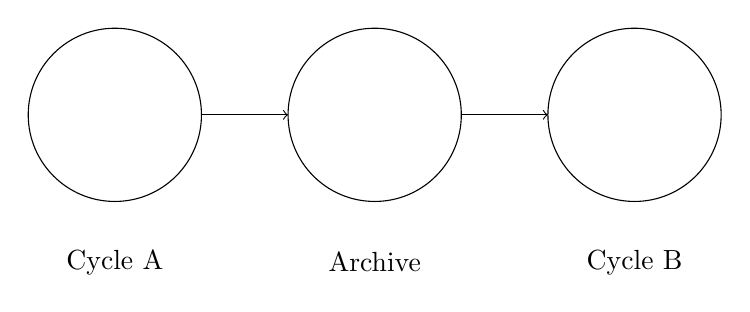
\begin{tikzpicture}[scale=1.1]
\draw (0,0) circle (1);
\draw (3,0) circle (1);
\draw (6,0) circle (1);

\draw[->] (1,0) -- (2,0);
\draw[->] (4,0) -- (5,0);

\node at (0,-1.7) {Cycle A};
\node at (3,-1.7) {Archive};
\node at (6,-1.7) {Cycle B};
\end{tikzpicture}
\end{center}

% =========================
\section{Conclusion}

The universe is framed as a memory-bearing geometric system: it explores difference locally, compresses it globally, and re-expresses inherited constraints across cycles.

\end{document}
